\documentclass[aspectratio=169,10pt]{beamer}
\usetheme[progressbar=frametitle,numbering=fraction]{metropolis}
\usepackage[utf8]{inputenc}
\usepackage{booktabs}
\usepackage{tikz}
\usetikzlibrary{arrows.meta,positioning,shapes.geometric,fit,backgrounds}
\usepackage{tcolorbox}

% ---------- colours ----------
\definecolor{cClaim}{HTML}{1D4ED8}
\definecolor{cObs}{HTML}{15803D}
\definecolor{cLim}{HTML}{B91C1C}
\definecolor{cAsm}{HTML}{B45309}
\definecolor{cBg}{HTML}{64748B}
\definecolor{cAnn}{HTML}{7E22CE}
\setbeamercolor{alerted text}{fg=cLim}

% ---------- evidence badges ----------
\newcommand{\badge}[2]{\tikz[baseline=(b.base)]\node[fill=#1,text=white,rounded corners=2pt,inner xsep=3pt,inner ysep=1.5pt,font=\scriptsize\bfseries](b){#2};}
\newcommand{\evcite}{\badge{cBg}{CITATION}}
\newcommand{\evarg}{\badge{cAsm}{ARGUMENT}}
\newcommand{\evqual}{\badge{cObs!75}{DATA, BY EYE}}
\newcommand{\evquant}{\badge{cObs}{DATA, NUMBERS}}
\newcommand{\evnone}{\badge{cLim}{NONE}}
\newcommand{\warn}{\textcolor{cLim}{\bfseries\(\triangle\)}}

\newtcolorbox{limbox}[1][]{colback=cLim!6,colframe=cLim,boxrule=0.6pt,arc=2pt,left=4pt,right=4pt,top=1pt,bottom=1pt,fonttitle=\bfseries\footnotesize,#1}
\newtcolorbox{evbox}[1][]{colback=cObs!6,colframe=cObs,boxrule=0.6pt,arc=2pt,left=4pt,right=4pt,top=1pt,bottom=1pt,fonttitle=\bfseries\footnotesize,#1}

\title{Lattice genome: the logic, the evidence, the limits}
\subtitle{Argument analysis of Wang, Calvat, Stinville \& Latypov, arXiv:2606.09611 (2026)}
\author{logprobe team -- Open Science Hackathon}
\date{21 October 2026}

\begin{document}

\maketitle

% =====================================================================
\begin{frame}[shrink=5]{The paper in one sentence}
\begin{center}
\large
VAE encodings of EBSD Kikuchi patterns (\emph{lattice genes}) are a valid ``materials gene'';
mapped over a sample (\emph{lattice genome}) they support visualization, segmentation and heterogeneity
quantification like conventional EBSD, with finer detail.
\end{center}
\vfill
\textbf{How to read the following slides.} Every step is tagged with the kind of evidence the paper gives for it:\\[4pt]
\evcite\ reference to prior work \quad
\evarg\ reasoning only \quad
\evqual\ figure judged visually \quad
\evquant\ numbers \quad
\evnone\ nothing shown
\\[6pt]
\warn\ marks where the evidence is weaker than the wording, \textcolor{cAnn}{purple} marks links \emph{we} add that the paper does not make.
\end{frame}

% =====================================================================
\begin{frame}{The argument at a glance}
\centering
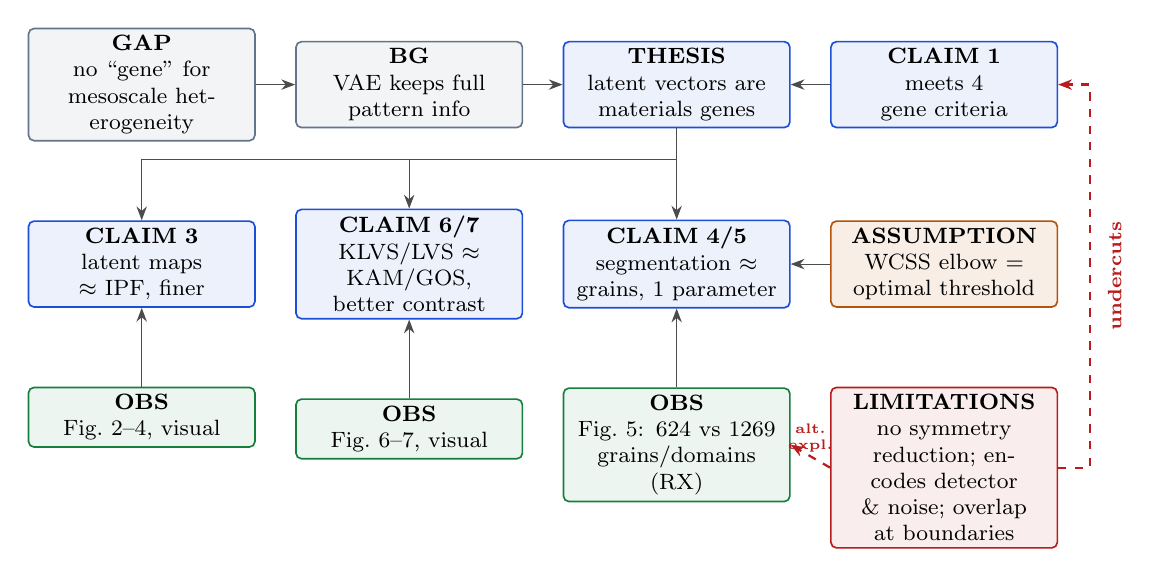
\begin{tikzpicture}[
  font=\footnotesize, >={Stealth[length=5pt]},
  box/.style={draw,rounded corners=2pt,align=center,minimum height=7mm,inner sep=2.5pt,line width=0.6pt},
  bg/.style={box,draw=cBg,fill=cBg!8,text width=27mm},
  cl/.style={box,draw=cClaim,fill=cClaim!8,text width=27mm},
  ob/.style={box,draw=cObs,fill=cObs!8,text width=27mm},
  li/.style={box,draw=cLim,fill=cLim!8,text width=27mm},
  as/.style={box,draw=cAsm,fill=cAsm!10,text width=27mm},
  sup/.style={->,draw=black!70},
  und/.style={->,dashed,draw=cLim,line width=0.8pt},
]
% row 1: motivation
\node[bg] (gap) {\textbf{GAP}\\no ``gene'' for mesoscale heterogeneity};
\node[bg,right=5mm of gap] (vae) {\textbf{BG}\\VAE keeps full pattern info};
\node[cl,right=5mm of vae] (thesis) {\textbf{THESIS}\\latent vectors are materials genes};
\node[cl,right=5mm of thesis] (crit) {\textbf{CLAIM 1}\\meets 4 gene criteria};
% row 2: tools
\node[cl,below=10mm of gap] (c3) {\textbf{CLAIM 3}\\latent maps $\approx$ IPF, finer};
\node[cl,right=5mm of c3] (c6) {\textbf{CLAIM 6/7}\\KLVS/LVS $\approx$ KAM/GOS, better contrast};
\node[cl,right=5mm of c6] (c4) {\textbf{CLAIM 4/5}\\segmentation $\approx$ grains, 1 parameter};
\node[as,right=5mm of c4] (asm) {\textbf{ASSUMPTION}\\WCSS elbow = optimal threshold};
% row 3: observations
\node[ob,below=10mm of c3] (o3) {\textbf{OBS}\\Fig.\ 2--4, visual};
\node[ob,below=10mm of c6] (o6) {\textbf{OBS}\\Fig.\ 6--7, visual};
\node[ob,below=10mm of c4] (o4) {\textbf{OBS}\\Fig.\ 5: 624 vs 1269 grains/domains (RX)};
\node[li,below=10mm of asm] (lim) {\textbf{LIMITATIONS}\\no symmetry reduction; encodes detector \& noise; overlap at boundaries};
% edges
\draw[sup] (gap) -- (vae);
\draw[sup] (vae) -- (thesis);
\draw[sup] (crit) -- (thesis);
\draw[sup] (thesis.south) -- ++(0,-4mm) -| (c3.north);
\draw[sup] (thesis.south) -- ++(0,-4mm) -| (c6.north);
\draw[sup] (thesis.south) -- ++(0,-4mm) -| (c4.north);
\draw[sup] (o3) -- (c3);
\draw[sup] (o6) -- (c6);
\draw[sup] (o4) -- (c4);
\draw[sup] (asm) -- (c4);
\draw[und] (lim.east) -- ++(4mm,0) |- node[pos=0.25,right,font=\scriptsize\bfseries,text=cLim,rotate=90,anchor=north,yshift=-1mm]{undercuts} (crit.east);
\draw[und] (lim.west) -- node[above,font=\tiny\bfseries,text=cLim,align=center,inner sep=1pt]{alt.\\expl.} (o4.east);
\end{tikzpicture}
\vfill
\scriptsize Blue: claims \quad Green: observations \quad Amber: assumption \quad Red: limitations (dashed = weakens a claim)
\end{frame}

% =====================================================================
\begin{frame}{Step 1 -- Motivation: why a ``lattice gene''?}
\begin{enumerate}\setlength\itemsep{4pt}
\item Materials Genome Initiative assumes an underlying ``code'' -- but what is a gene? \hfill \evcite\ [1,2]
\item Billinge: a gene must be \emph{compact, unique, measurable, with a similarity metric} \hfill \evcite\ [3]
\item Pair distribution functions meet this, but carry no spatial information \hfill \evcite\ [3]
\item Spatial heterogeneity (phases, grains, defects) controls alloy properties \hfill \evcite\ [4,5]
\item[$\Rightarrow$] \textbf{Gap:} no gene concept for mesoscale heterogeneous materials \hfill \evarg
\item EBSD maps Kikuchi patterns at the mesoscale, but reduces them to lossy descriptors \hfill \evcite\ [6--15]
\item A VAE compresses a pattern into a vector that can reconstruct it \hfill \evcite\ [15,26--28]
\item[$\Rightarrow$] \textbf{Thesis:} VAE latent vector $=$ lattice gene; map of them $=$ lattice genome
\end{enumerate}
\vfill
\small The motivation is coherent and well referenced. The gap statement rests on argument only (no survey).
\end{frame}

% =====================================================================
\begin{frame}{Step 2 -- Does the latent vector meet the gene criteria?}
\small
\begin{tabular}{@{}p{0.2\linewidth}p{0.38\linewidth}p{0.12\linewidth}p{0.24\linewidth}@{}}
\toprule
\textbf{Criterion} & \textbf{Paper's support} & \textbf{Evidence} & \textbf{Gap}\\
\midrule
Compact & latent vector is low-dimensional & \evarg & \warn\ size ratio never given\\[3pt]
Accessible & one forward pass of a pretrained encoder & \evarg & --\\[3pt]
Distance metric & latent distance reflects lattice similarity & \evarg & \warn\ never tested; contradicted later\\[3pt]
Near-unique & pattern reconstructable $\Rightarrow$ unique lattice state & \evarg\ \evcite & \warn\ reconstruction error not reported\\
\bottomrule
\end{tabular}
\vfill
\begin{limbox}[title=Logical issue]
The abstract says \emph{``We show that this representation satisfies key criteria''} -- but Sec.~2 contains no new data.
Reconstruction proves the code determines the \emph{pattern}, not that the pattern uniquely determines the \emph{lattice state}.
\end{limbox}
\end{frame}

% =====================================================================
\begin{frame}[shrink=5]{Step 3 -- Tool 1: latent component maps}
\begin{columns}[T]
\begin{column}{0.56\textwidth}
\includegraphics[width=\linewidth]{figs/fig2.png}\\[-2pt]
{\tiny Fig.~2 of the paper: (a) IPF, (b) latent component maps, (c) explained variance, (d) close-ups.}
\end{column}
\begin{column}{0.42\textwidth}
\footnotesize
\textbf{Method:} PCA of 127-d lattice genes, PC1--3 $\to$ RGB.\\[4pt]
\begin{evbox}[title=Evidence]
\begin{itemize}\setlength\itemsep{0pt}\setlength\topsep{0pt}
\item Same grain structure as IPF \hfill\evqual
\item Extra features: prep.\ damage, extra grain, gradients, cells (``likely'') \hfill\evqual
\item PC1--3 explain 25--37\,\%; $\sim$20 PCs for $\sim$100\,\% \hfill\evquant
\end{itemize}
\end{evbox}
\begin{limbox}[title=Limits]
\begin{itemize}\setlength\itemsep{0pt}\setlength\topsep{0pt}
\item Colours not transferable between maps (authors)
\item ``Finer features'' interpreted as ``likely'' physics, not checked independently
\end{itemize}
\end{limbox}
\end{column}
\end{columns}
\end{frame}

% =====================================================================
\begin{frame}[shrink=5]{Step 4 -- Tool 2: segmentation in latent space}
\begin{columns}[T]
\begin{column}{0.5\textwidth}
\includegraphics[width=\linewidth,height=0.72\textheight,keepaspectratio]{figs/fig5.png}\\[-2pt]
{\tiny Fig.~5: boundary overlay (pink: latent domains, black: 5° grains) and area distributions.}
\end{column}
\begin{column}{0.48\textwidth}
\footnotesize
\textbf{Method:} merge neighbours if latent angle \emph{and} distance $<$ the $p$-th percentile; $p$ chosen at the WCSS ``elbow''.\\[3pt]
\begin{evbox}[title=Evidence]
\centering
\begin{tabular}{lrrr}
 & RX & W & AM\\\midrule
grains (5°) & 624 & 3314 & 1326\\
domains & 1269 & 3634 & 3143\\
$p^*$ & 76 & 80 & 73\\
\end{tabular}\\[2pt]
\raggedright boundaries ``largely coincide'' \evqual\ \; counts \evquant
\end{evbox}
\begin{limbox}[title=Limits]
\begin{itemize}\setlength\itemsep{0pt}
\item Elbow $=$ optimum is \emph{assumed}; constants (60--95, 10\,\%, 3 steps) ad hoc \hfill\evnone
\item Some real grain boundaries are missed
\item ``Generalizes to any EBSD dataset'' from $n=3$
\end{itemize}
\end{limbox}
\end{column}
\end{columns}
\end{frame}

% =====================================================================
\begin{frame}[shrink=5]{Step 5 -- Tool 3: heterogeneity metrics KLVS and LVS}
\begin{columns}[T]
\begin{column}{0.55\textwidth}
\includegraphics[width=\linewidth]{figs/fig6.png}\\[-2pt]
{\tiny Fig.~6: (a) KAM, 0--8°; (b) KLVS, 0--120°.}
\end{column}
\begin{column}{0.43\textwidth}
\footnotesize
\textbf{Method:} KLVS = mean latent angle to neighbours (KAM analog); LVS = mean angle to domain centroid (GOS analog).\\[3pt]
\begin{evbox}[title=Evidence]
\begin{itemize}\setlength\itemsep{0pt}\setlength\topsep{0pt}
\item Same qualitative trends as KAM/GOS \hfill\evqual
\item Indexing artifacts and a scratch weaker in KLVS \hfill\evqual
\item Substructure in AM grains visible \hfill\evqual
\end{itemize}
\end{evbox}
\begin{limbox}[title=Limits]
\begin{itemize}\setlength\itemsep{0pt}\setlength\topsep{0pt}
\item ``Better contrast'' never quantified
\item Values not comparable (no symmetry reduction)
\item LVS on \emph{domains} vs GOS on \emph{grains}: two changes at once
\end{itemize}
\end{limbox}
\end{column}
\end{columns}
\end{frame}

% =====================================================================
\begin{frame}{Limitations the authors state (Sec.~5)}
\begin{enumerate}\setlength\itemsep{6pt}
\item \textbf{Dataset-dependent colours.} PCA per map, so latent maps are not comparable across samples.
\item \textbf{No explicit crystal symmetry.} Latent angles are not reduced by symmetry, hence KLVS/LVS $\gg$ KAM/GOS and no quantitative match.
\item \textbf{Measurement leaks into the gene.} Detector geometry, pattern centre, background and noise are encoded too (one of the 128 dimensions was even dropped for tracking geometry).
\item \textbf{Overlapping patterns at boundaries.} A gene there encodes a mixture of lattices; this partly explains the extra domain boundaries.
\end{enumerate}
\vfill
\small The authors propose physically constrained encoders and larger training sets as remedies \evcite\ [40--42] -- not demonstrated.
\end{frame}

% =====================================================================
\begin{frame}{Limitations the paper does \emph{not} connect}
\begin{limbox}[title={1. Its own limitations undercut the gene criteria}]
\small Limitations 2 and 3 mean latent distance reflects \emph{symmetry setting and measurement}, not only lattice similarity --
yet ``distance metric reflecting structural similarity'' is claimed as satisfied (Sec.~2, Conclusion).
\textcolor{cAnn}{(link added by us)}
\end{limbox}
\begin{limbox}[title={2. Validation that cannot fail}]
\small Agreement with conventional EBSD $\Rightarrow$ ``validated''; disagreement $\Rightarrow$ ``more sensitive''.
No independent ground truth (HR-EBSD, ECCI, TEM, synthetic patterns) distinguishes real substructure from artifacts.
Limitation 4 offers an alternative explanation for the extra domains.
\end{limbox}
\begin{limbox}[title={3. Scope vs.\ generality}]
\small 3 maps, 2 alloys, all FCC Ni-base, one encoder (training data not stated), code ``upon acceptance''.
Claims: ``readily generalizes to any EBSD dataset'', works for hard-to-index and multiphase patterns, ``will remain applicable''.
\end{limbox}
\end{frame}

% =====================================================================
\begin{frame}{Conclusion claims vs.\ their weakest support}
\small
\begin{tabular}{@{}p{0.43\linewidth}p{0.17\linewidth}p{0.34\linewidth}@{}}
\toprule
\textbf{Conclusion states \dots} & \textbf{Evidence} & \textbf{Weakest link}\\
\midrule
lattice gene satisfies Billinge's criteria & \evarg & untested; undercut by own limitations\\
extends MGI to the mesoscale & \evarg & analogy only\\
latent maps reveal subtler variations & \evqual & ``likely'' interpretations\\
segmentation consistent with grain maps & \evqual\ \evquant & no overlap metric; no ground truth\\
spreads recover trends ``with better contrast'' & \evqual & shown by eye, for KLVS only\\
works without indexing & \evarg & not tested on hard-to-index data\\
remains applicable as encoders evolve & \evarg & forward-looking\\
\bottomrule
\end{tabular}
\vfill
\begin{tcolorbox}[colback=cClaim!6,colframe=cClaim,boxrule=0.6pt,arc=2pt]
\small\textbf{Bottom line.} Clear concept and well-described tools; the language (``we show'', ``validated'', ``objective'', ``any dataset'')
is stronger than the evidence: argument for the core claim, visual agreement for the tools, $n=3$ for generality.
\end{tcolorbox}
\end{frame}

% =====================================================================
\begin{frame}{What would close the gaps}
\begin{itemize}\setlength\itemsep{6pt}
\item \textbf{Test the metric:} latent distance vs.\ misorientation and GND density on the same pixels.
\item \textbf{Report the reconstruction error} and the compression ratio.
\item \textbf{Ground truth for ``finer details'':} correlate extra domains with HR-EBSD/ECCI, or use synthetic patterns with known defects.
\item \textbf{Quantify agreement:} boundary overlap (precision/recall), contrast-to-noise of KLVS vs.\ KAM.
\item \textbf{Separate the effects:} compute LVS on the conventional grains as well.
\item \textbf{Widen the scope:} BCC/HCP, multiphase, a second detector; release code.
\end{itemize}
\vfill
\scriptsize Full machine-readable argument chain: \texttt{logprobe/data/wang2026\_lattice\_genome.yaml} (66 statements, 65 relations).
\end{frame}

\end{document}
